In this section we look at the results of the perceptual test and analyze them.

\subsubsection{Outliers}
\begin{figure}[htb!]
	\centering
	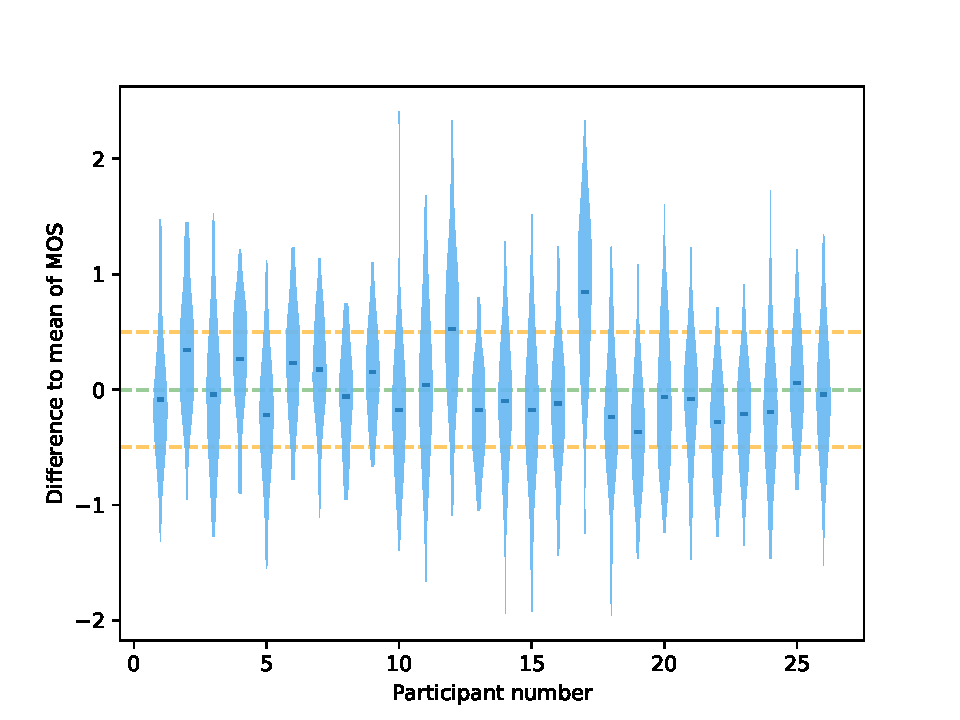
\includegraphics[width=3in]{participant_mos_violin}
	\caption{Difference between average MOS and the invididual ratings for each participant}
	\label{fig:result:participant_violin}
\end{figure}

We calculated the average of all \textit{MOS} and compared the differences of each participants ratings to the average. This can be seen in \ref{fig:result:participant_violin}. All participants apart from number 12 and 17 fall into a difference range of $[-0.5, 0.5]$ to the mean. For this reason we exclude the rating data of participants 12 and 17 from our further analysis.





\subsubsection{\textit{MOS} per Sequence}
\begin{figure}[htb!]
	\centering
	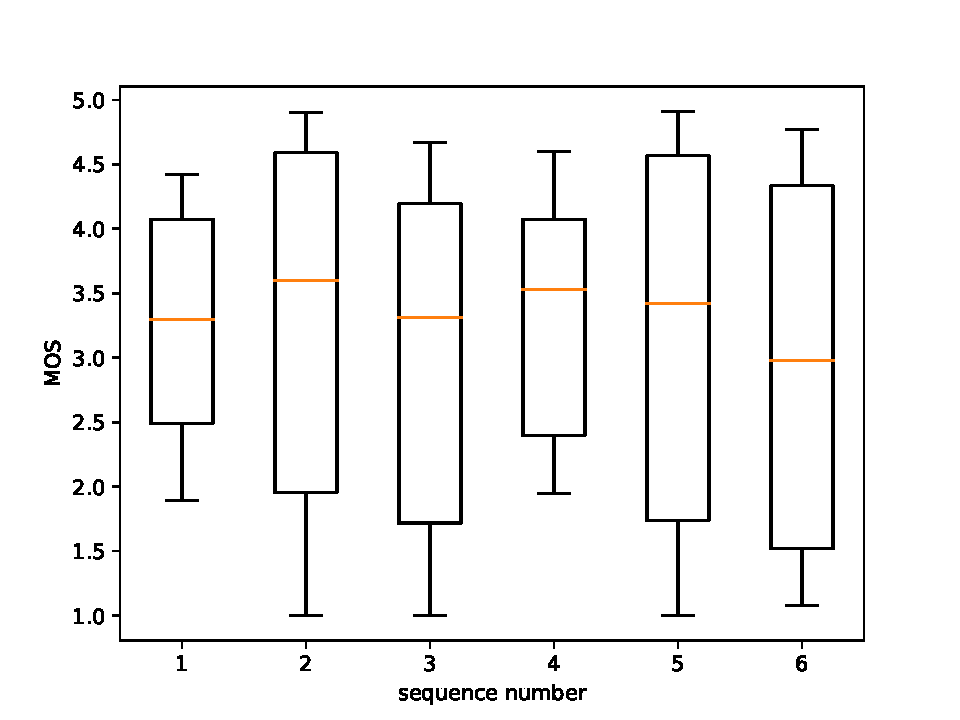
\includegraphics[width=3.5in]{mos_per_sequence}
	\caption{\textit{MOS} distribution per sequence over all versions of the sequence - 1: Air Show, 2: Big Buck Bunny, 3: Fjord, 4: Moment of Intensity, 5: Snow Monkeys, 6: Streets of India}
	\label{fig:result:mos_per_sequence}
\end{figure}

In Figure \ref{fig:result:mos_per_sequence} we show the \textit{MOS} for each sequence aggregated over all versions of this sequence. We see that the distributions are similar over all sequences and that every sequence has ratings on all steps of the \textit{ACR} (Absolute Category Rating) scale. This suggests a broad range of qualities in the encoded video.




\subsubsection{\textit{MOS} per Preset}
\begin{figure*}[htb!]
	\centering
	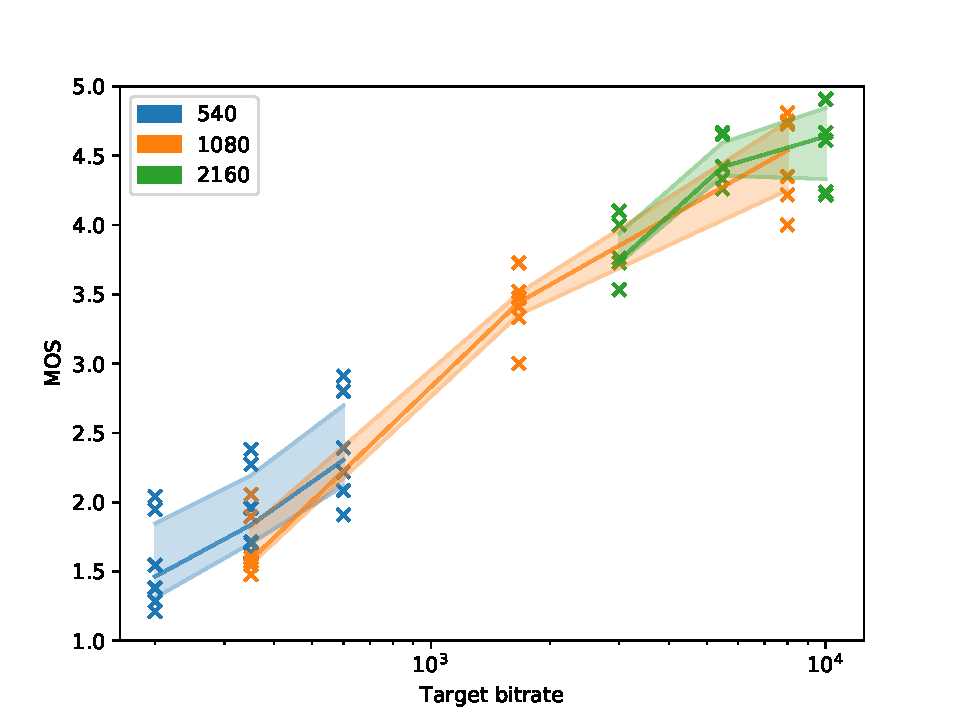
\includegraphics[width=3.45in]{correlation_bitrate_mos_p1}
	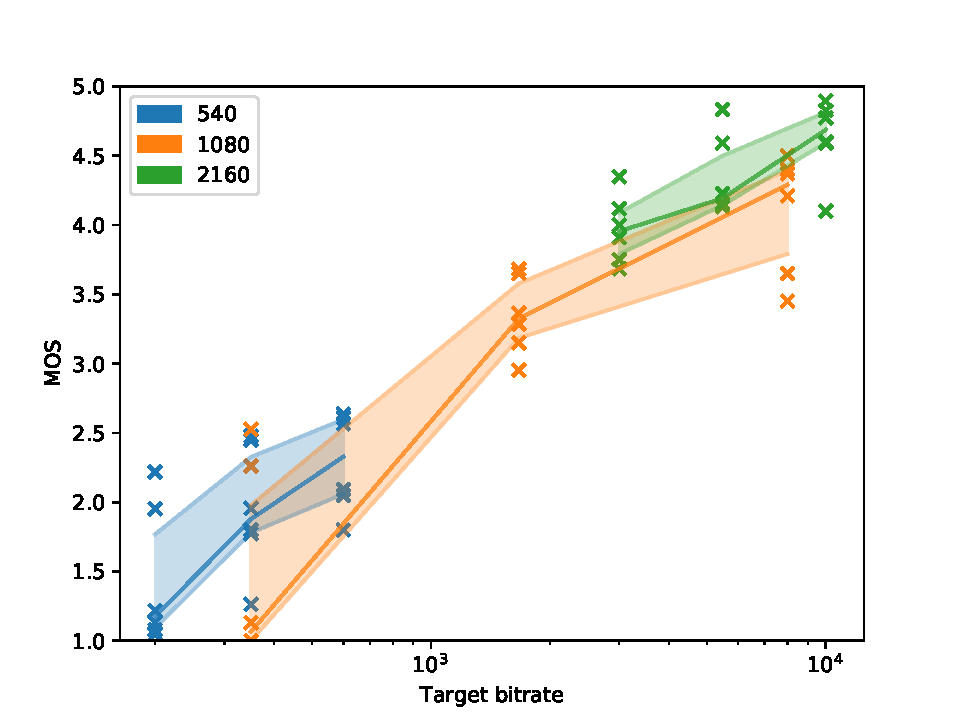
\includegraphics[width=3.45in]{correlation_bitrate_mos_p2}
	\caption{Correlation between bitrate and \textit{MOS} for both encoding presets. The center line represents a median and the outer line the 25th and 75th percentile of \textit{MOS} for the 6 sequences.}
	\label{fig:result:correlation_bitrate_mos}
\end{figure*}

The Distribution of \textit{MOS} values for each preset at different resolutions is shown in Figure \ref{fig:result:correlation_bitrate_mos}.
The "expert" preset quality is higher at 2160p resolution compared to the other preset and also compared to 1080p. For high and medium bitrates at 1080p and 540p the quality is similar to preset 1, but the MOS values exhibit a wider spread.
However, we see that especially for the lowest bitrate version the quality of "expert" preset (2) degrades, which we could already predict from our \textit{VMAF} scores after encoding in Fig. \ref{fig:vmaf:encoded}.

\begin{figure}[htb!]
	\centering
	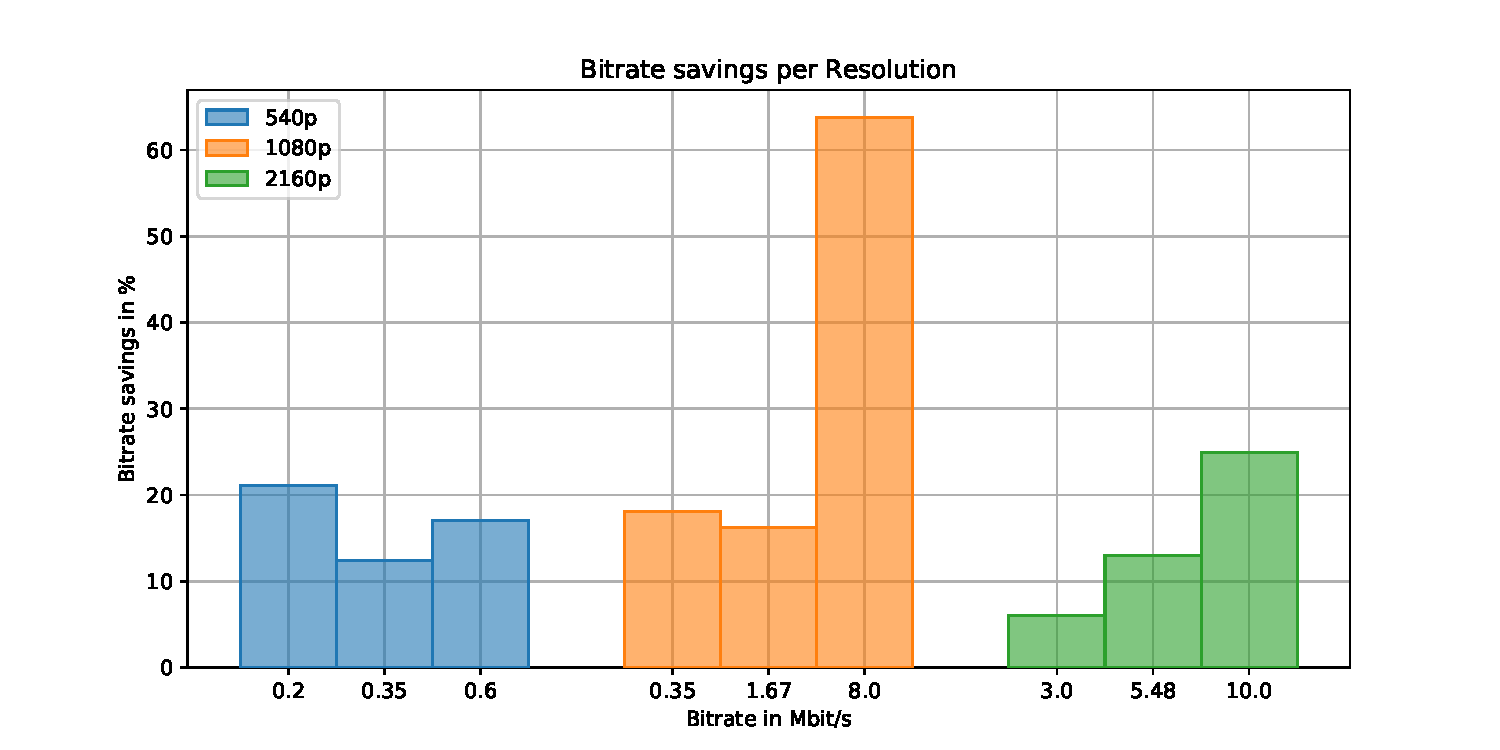
\includegraphics[width=3.5in]{bitrate_savings}
	\caption{Relative bitrate difference of "expert" preset compared to "na\"{\i}ve" preset at all target bitrates. For target bitrates with added hatching the "expert" preset MOS is smaller than the "na\"{\i}ve" preset MOS.}
	\label{fig:result:bitrate_savings}
\end{figure}
\begin{figure}[htb!]
	\centering
	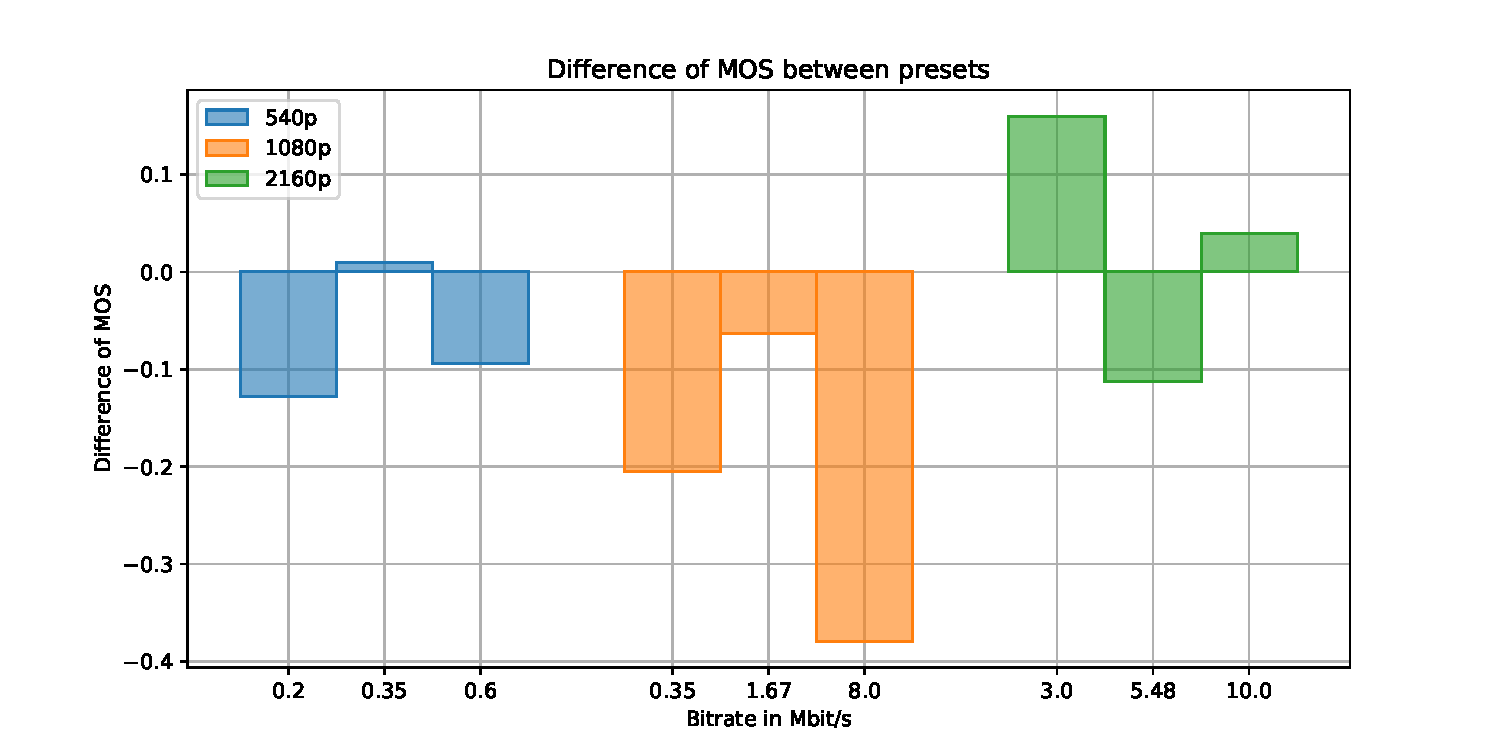
\includegraphics[width=3.5in]{quality_difference}
	\caption{}
	\label{fig:result:quality_difference}
\end{figure}

We further look at the bitrate differences between the presets in Figure \ref{fig:result:bitrate_savings}. It shows the relative bitrate savings for each target bitrate. The hatched bars show where the "expert" preset degrades the subjective quality below that of , which happens mainly for the 540p and 1080p resolutions. The 2160p versions of the content largely benefit from the "expert" preset with high subjective quality at significantly lower bitrates.


\begin{figure}[htb!]
	\centering
	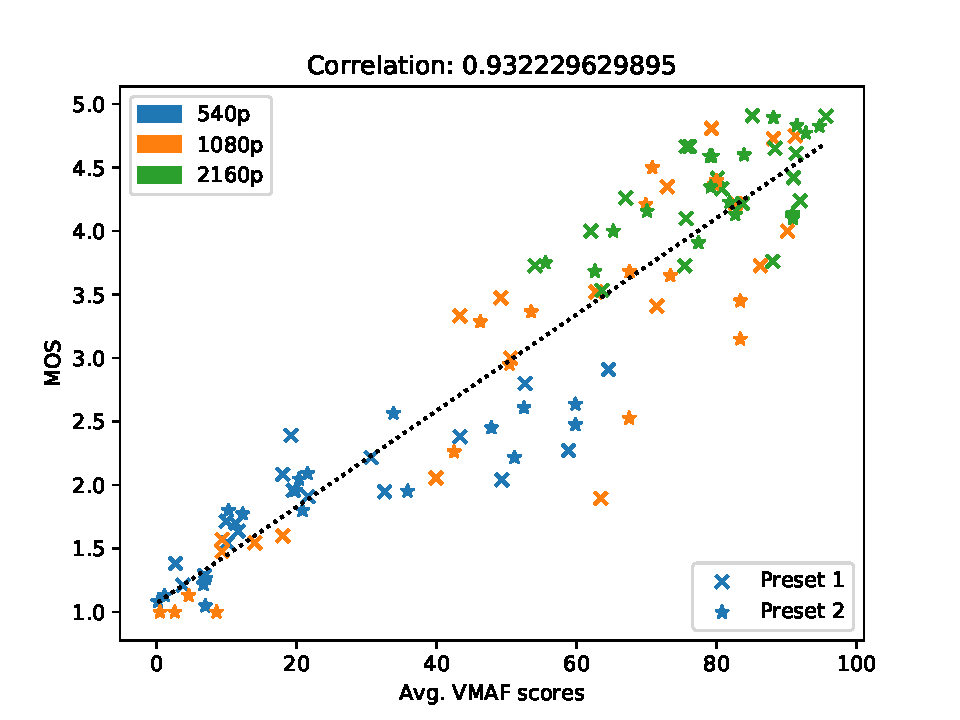
\includegraphics[width=3in]{correlation_vmaf_mos}
	\caption{Correlation between average \textit{VMAF} scores and \textit{MOS} for each preset and resolution}
	\label{fig:result:correlation_vmaf_mos}
\end{figure}

The Pearson product-moment correlation between user-rating based \textit{MOS} and the precomputed \textit{VMAF} scores is strong at 93\% (see fig. \ref{fig:result:correlation_vmaf_mos}).
\\
